\question TCP报文的数据部分最大长度为
\par\twoch{64KB-20B}{1500B-40B}{\textcolor{red}{64KB-40B}}{1500B-20B}
\begin{solution}因为IP数据报的总长度为16位,所以最大总长度为2\^{}16B=64KB,又TCP、IP的首部分别为20B,所以TCP报文的数据部分最大长度为64KB-40B。
可能疑问点:以太网数据链路层包含首部与尾部的最大帧长也就1518B,TCP报文的数据部分最大长度怎么可能达到64KB-40B?或者说为什么IP数据报的最大总长度可以达到2\^{}16=64KB?为什么有些书上说TCP报文段的数据部分不会超过1460B?
解析:IP地址的总长度为16位,也许是以前以太网还没有诞生前规定的,所以才造成IP数据报的总长度理论上最大可以达到2\^{}16=64KB。但是在以太网中,一般IP数据报的长度不会超过1500B(包含IP分组首部),因为超过这么长到了数据链路层就需要分片,会造成麻烦。所以,不少书中也会默认TCP报文段的数据部分不会超过1460B(因为TCP报文首部可达到40B,1500B-40B=1460B)。
\end{solution}
\question 以太网的数据帧封装如图3-2所示,包含的TCP段中的数据部分最长应该是( ~)

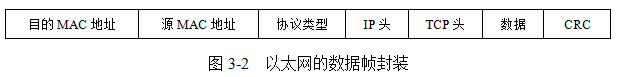
\includegraphics[width=3.33333in,height=0.40625in]{computerassets/25d66fd7ecf9a4aa73d66c4295ed68fb.png}
\par\twoch{1434}{\textcolor{red}{1460}}{1480}{1500}
\begin{solution}以太网帧数据域最大长度为1500B,而IP头和TCP头字段最小长度为20B。因此,用户数据最长为(1500-20-20)B=1460B。
\end{solution}
